\documentclass[12pt]{article}

\usepackage{graphicx}
\graphicspath{ {./images/} }
\usepackage{amsmath}

\renewcommand{\=}{\quad = \quad}
\newcommand{\+}{\; + \;}

\begin{document}
	
	\section{introduction}
	
	This example emulates a running shower fed by a water tank.
	When hot water is extarcted from the tank to the shower, new cold water is injected into the tank, thus making the tank water temperature drop.
	The water tank is provided with a sensor measuring the water temperature and a heater able to heat the water.
	However, the sensor comes with a small delay, wich can be tuned in the settings.\\
	
	To understand the need for a PID controller, we can first try a more basic approach, using the "basic" mode.
	In this mode, if the sensed temperature is below the target, the heater starts, else the heater shuts off.
	By using this mode, we see that the sensor realizes too late that the temperature is below target, and realized to late that the temperature is above target.
	Thus we obtain an unconfortable oscillation of the temperature around the target which would not provide a great shower experience.
	However, we see that when we switch to the PID mode, that oscillation disapears quickly and the temperature stabilizes around the target much better,
	that is if and only if the PID parameters (Kp, Ki, Kd, Tau) are well calibrated off course.\\
	
	To understand why the PID controller works so much better than the basic mode, we can see it as follows :
	In the basic mode, only the current state of the sensor is taken into account.
	Whereas in the PID mode, the current state of the sensor is taken into account through the proportional term (Kp),
	but also the past states off the sensor are accounted for through the integral term (Ki),
	aswell as the predicted futur state of the sensor through the derivative term (Kd).
	Altogether, this makes for a much better controller.
	
	\newpage
	
	\section{diagrams}
	


	\begin{figure}[h]
		\centering
		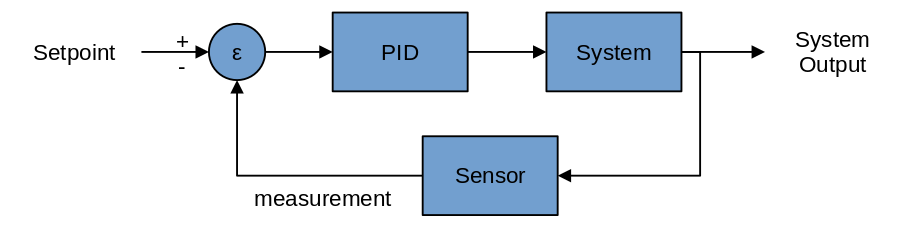
\includegraphics[scale=0.4]{PID.png}
		\caption{PID block diagram}
	\end{figure}

	\begin{figure}[h]
		\centering
		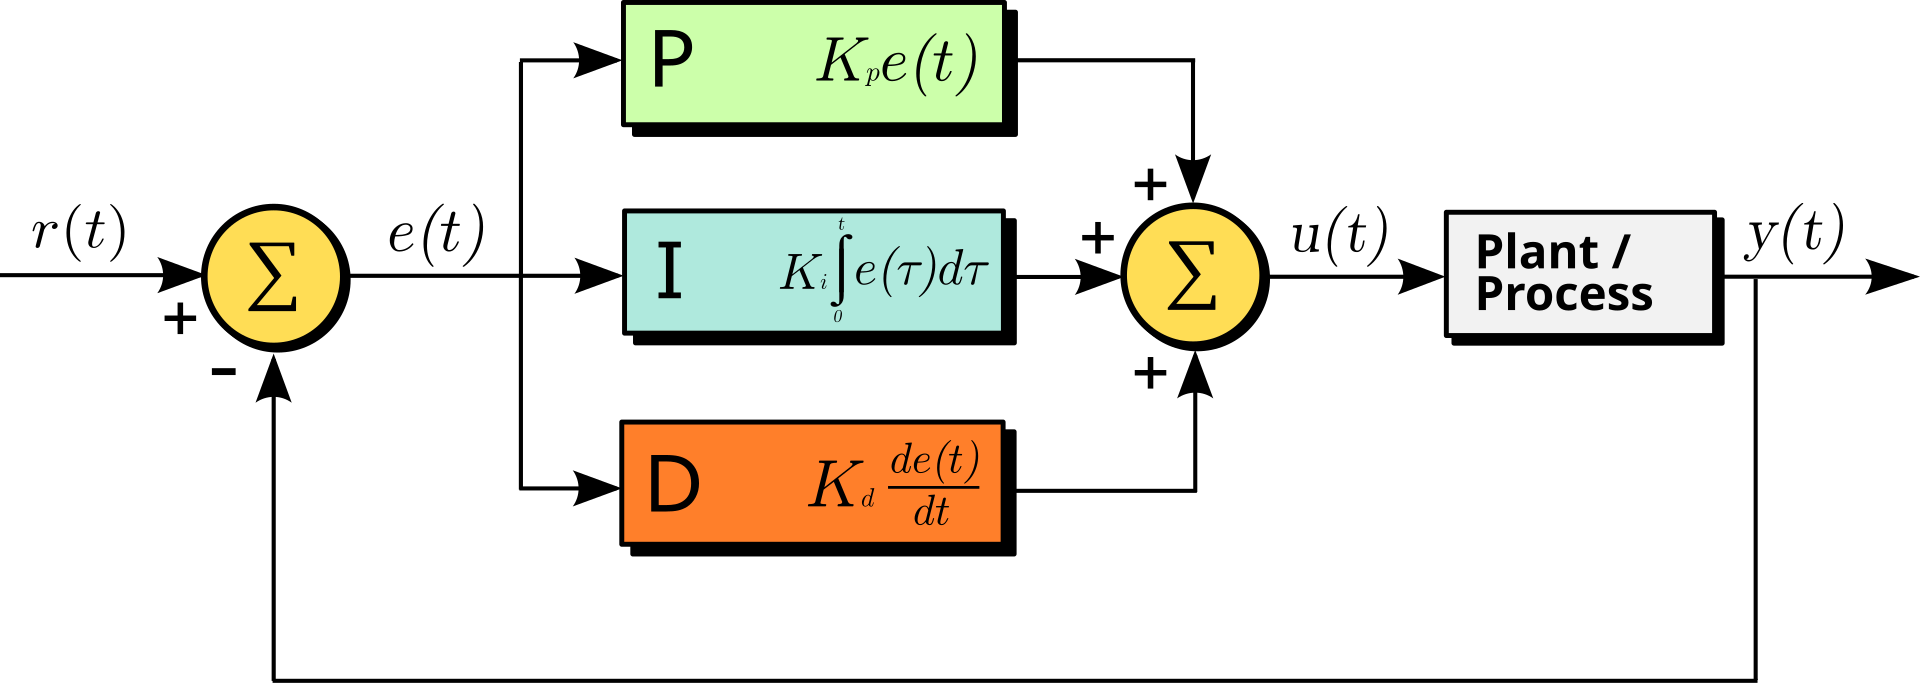
\includegraphics[scale=0.15]{PID2.png}
		\caption{PID Block Diagram, Arturo Urquizo, CC BY-SA 3.0 via Wikimedia Commons}
	\end{figure}

\newpage

	\section{math}
	
	from the block diagram, we get the following equation
	
	$$ u(t) \= K_p e(t) \+ Ki \int_0^t e(\tau) d \tau \+ K_d \frac{de(t)}{dt} $$
	
	in the continuous domain, this equation becomes
	
	$$
	\bar{u} (s) \= K_p \bar{e} (s) \+ K_i \frac{1}{s} \bar{e} (s) \+ K_d s \bar{e} (s)
	$$
	
	But because the derivative of an impulse is infinte, thiscan produce kicks in the response, hence, a low pass filter can be added to the derivative term as such
	
	$$
	\bar{u} (s) \= K_p \bar{e} (s) \+ K_i \frac{1}{s} \bar{e} (s) \+ K_d \frac{s}{s \tau + 1} \bar{e} (s)
	$$
	
	using the Tustin transform $ s \rightarrow \frac{2}{T} \frac{z-1}{z+1} $ and the following property $ \bar{y} (z) = \bar{x} (z) . z^{-1} \rightarrow y[n] = x[n-1]$, we can convert this equation from continuous to discrete domain, or s-domain to z-domain.
	
	We then get the following equations
	
	\begin{flalign}
		& p[n] = K_p e[n] \\
		& i[n] = \frac{K_i T}{2} (e[n] + e[n-1]) + i[n-1] \\
		& d[n] = \frac{2 K_d}{2 \tau + T} (e[n] - e[n-1]) + \frac{2 \tau - T}{2 \tau + T} d[n-1] \\
		& u[n] = p[n] + i[n] + d[n]
	\end{flalign}
	
	
	
	
\end{document}